\documentclass[a4paper]{article}
\usepackage[utf8]{inputenc}
\usepackage[spanish, es-tabla, es-noshorthands]{babel}
\usepackage[table,xcdraw]{xcolor}
\usepackage[a4paper, footnotesep = 1cm, width=20cm, top=2.5cm, height=25cm, textwidth=18cm, textheight=25cm]{geometry}
%\geometry{showframe}

\usepackage{tikz}
\usepackage{amsmath}
\usepackage{amsfonts}
\usepackage{amssymb}
\usepackage{float}
\usepackage{graphicx}
\usepackage{caption}
\usepackage{subcaption}
\usepackage{multicol}
\usepackage{multirow}
\setlength{\doublerulesep}{\arrayrulewidth}
\usepackage{booktabs}

\usepackage{hyperref}
\hypersetup{
    colorlinks=true,
    linkcolor=blue,
    filecolor=magenta,      
    urlcolor=blue,
    citecolor=blue,    
}

\newcommand{\quotes}[1]{``#1''}
\usepackage{array}
\newcolumntype{C}[1]{>{\centering\let\newline\\\arraybackslash\hspace{0pt}}m{#1}}
\usepackage[american]{circuitikz}
\usetikzlibrary{calc}
\usepackage{fancyhdr}
\usepackage{units} 

\graphicspath{{../Ejercicio-1/}{../Ejercicio-2/}{../Ejercicio-3/}{../Ejercicio-4/}}

\pagestyle{fancy}
\fancyhf{}
\lhead{22.01 Teoría de Circuitos}
\rhead{Mechoulam, Lambertucci, Rodriguez Turco, Londero, Galdeman}
\rfoot{\centering \thepage}
\begin{document}

\subsection{Introducción}
En esta sección se implementará un oscilador de Wien, el cual se basa en el criterio de Barkhausen para funcionar.
\subsection{Oscilador de Wien.}
El oscilador de Wien es un oscilador que permite generar señales senoidales de un amplio espectro de frecuencias, desde 5Hz hasta aproximadamente 1MHz.
Para lograr esto cuenta con una retroalmientación positiva y negativa. Con la particularidad que en el lazo de retroalimentación positiva utiliza una resistencia dinámica.
Un factor vital para que el oscilador funcione, es la correcta utilización del criterio de Barkhausen, el mismo dice que dado un sistema realimentado, la ganancia del lazo debe ser unitaria para una cierta frecuencia f, única frecuencia a la cual el amplificador realimentado será inestable.
A continuación se procederá a analizar el circuito propuesto por la cátedra.
\begin{figure}[H]
	\centering
	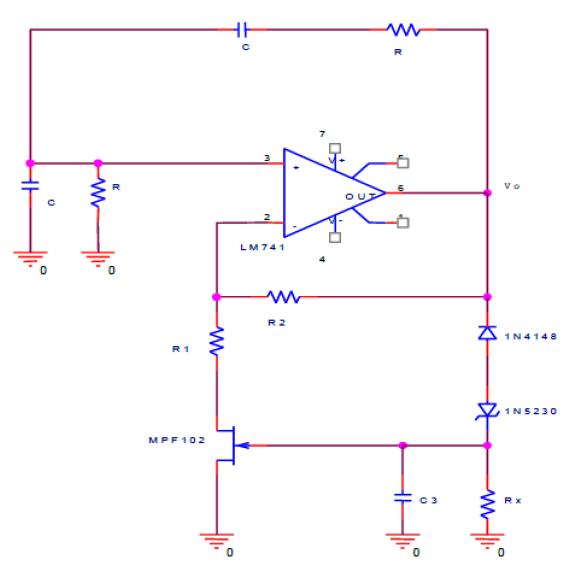
\includegraphics[width=0.5\textwidth]{Imagenes-Ej1/oscCatedra.PNG}
	\label{fig:cirosc}
	\caption{Oscilador de Wien}
\end{figure}

\subsubsection{Cálculo analítico}
Para el análisis se observo que existen 3 secciones bien definidas, siendo estas la realimentación positiva, la realimentación negativa y el AGC (Automatic Gain Control).
\begin{figure}[H]
	\centering
	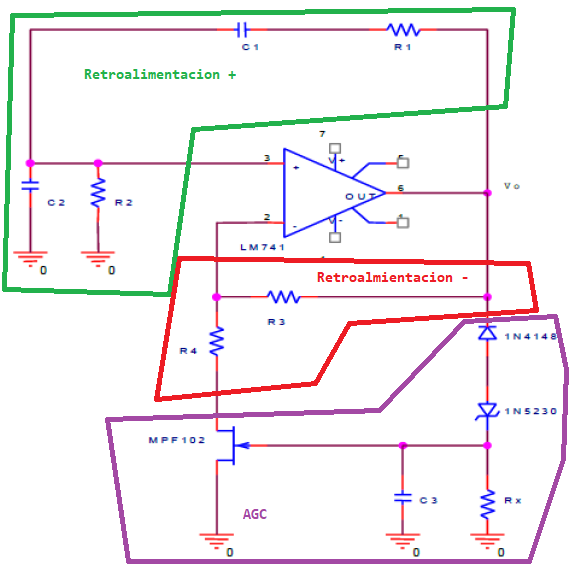
\includegraphics[width=0.5\textwidth]{Imagenes-Ej1/oscCatedraEtapas.PNG}
	\label{fig:cirosc}
	\caption{Oscilador de Wien separado por etapas.}
\end{figure}

\subsubsection{Singularidades}
\subsection{Elecciones de diseño.}
\subsection{Simulaciones.}
\subsection{Mediciones.}
\subsection{Análisis de Resultados.}
\subsection{Conclusiones.}
%\begin{figure}[H]
%	\centering
%	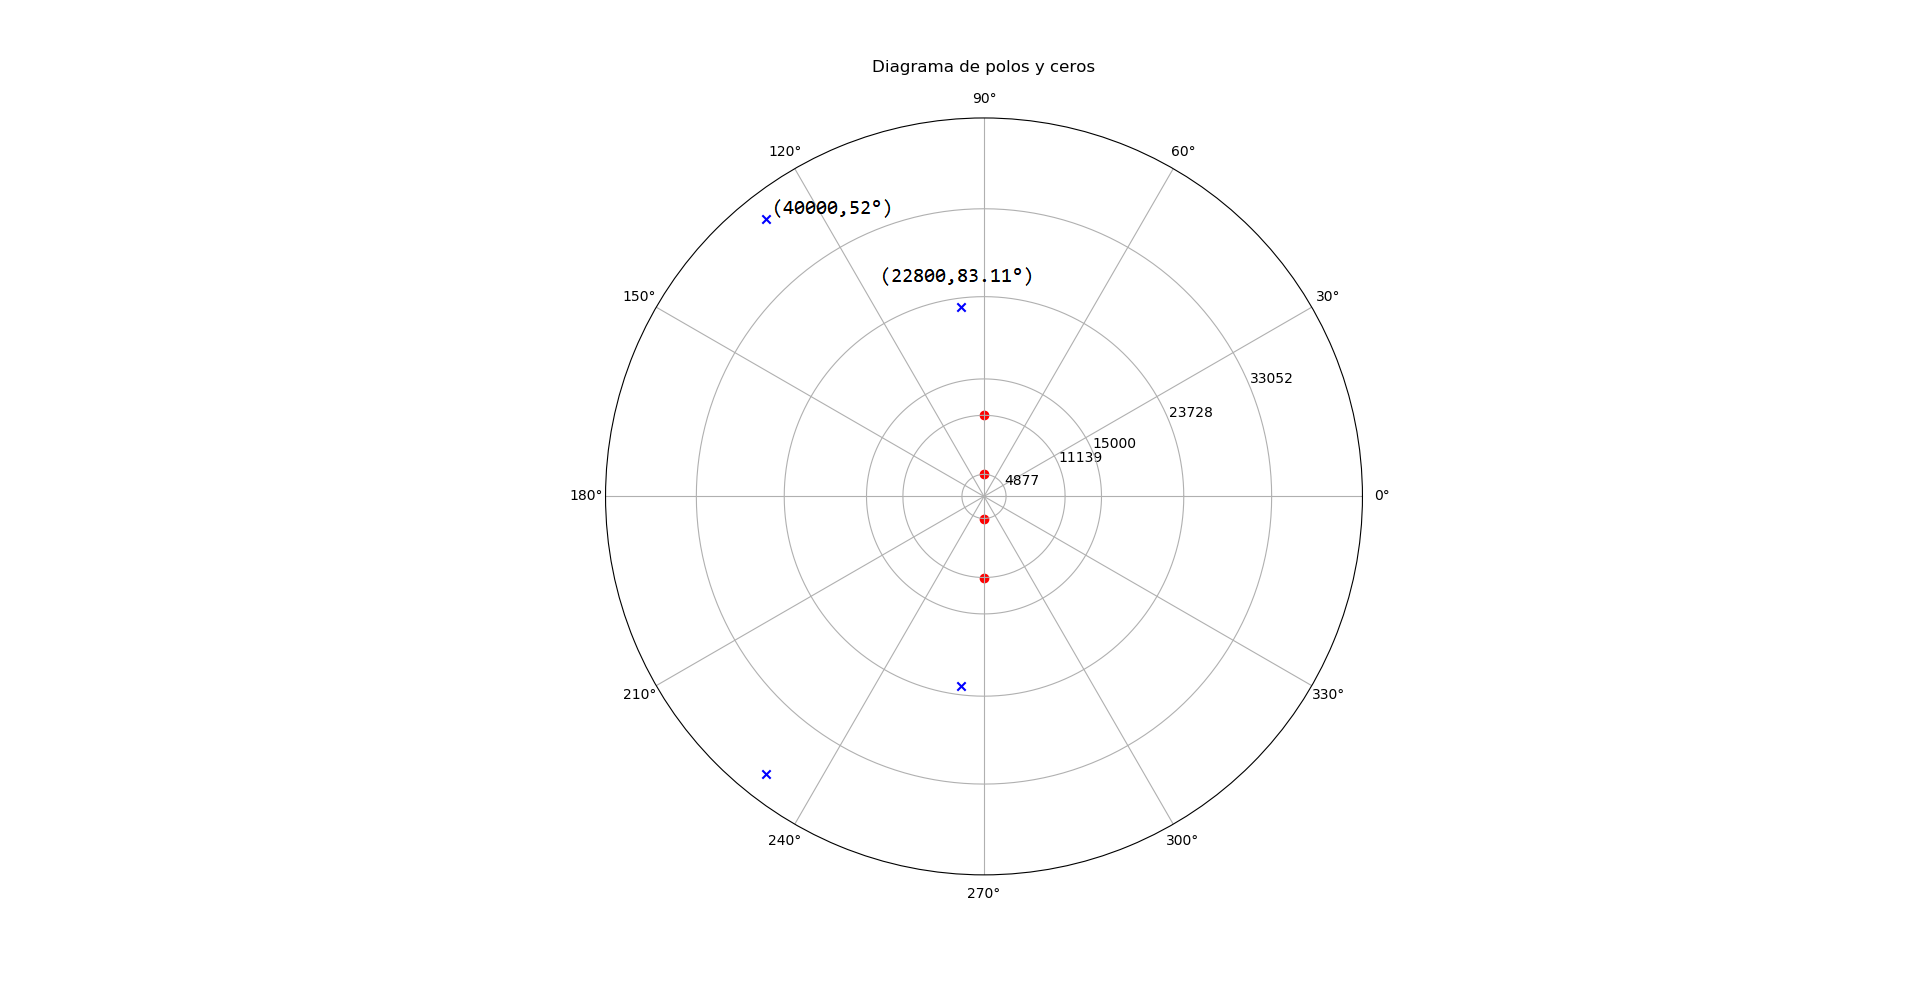
\includegraphics[width=\textwidth]{Imagenes-Ej3/DiagramaPolosYCeros.png}
%	\label{fig:poleZeroDiag}
%	\caption{Diagrama Polos y Ceros}
%\end{figure}


\end{document}